\subsection{Mixing length theory}
Heat (and mass) transport for both the viscous (solid-state) and inviscid regime is parameterised using \textbf{mixing length theory}.  1-D thermal evolution can be effectively modelled using mixing length theory to approximate the radially averaged results of full 3-D convective simulations.  The physical picture is that convective heat transport at a distance $l$ from the nearest boundary is dominated by fluid parcels of size $l$, which transport heat vertically over a distance equal to their size before they dissipate.  The sensible heat flux is expressed as a sum of conductive and convective terms:
\begin{equation}
J_q = -\rho C_p \kappa \left( \frac{\partial T}{\partial r} \right)_S - \rho C_p \kappa_{\rm h}\Delta (\delta_r T)_S
\label{eqn:Jq}
\end{equation}
where $r$ is the radius, $\kappa$ is the thermal diffusivity (due to conduction), $\kappa_{\rm h}$ is the eddy diffusivity (due to convection), and the thermal gradient relative to the adiabat is given by:
\begin{equation}
\label{eqn:thermgrad}
\Delta (\delta_r T)_S =  \frac{\partial T}{\partial r} - \left( \frac{\partial T}{\partial r} \right)_S 
\end{equation}
Equation \ref{eqn:Jq} is cast in a diffusive form identical to Fourier's Law, where the adiabatic thermal gradient transports heat according to simple conduction, and the deviation from the adiabat carries heat diffusively through either conduction, viscous convection, or inviscid convection, as appropriate (for details, see section \ref{sec:mixinglenth} below).

The effective convective diffusivity is expressed in a form identical to Fourier's law (formerly called the eddy diffusivity according to Abe 1993), is determined from the mean free path by $\kappa \sim v l$:
\begin{equation}
  \kappa_{\rm conv} = \begin{cases}
  0 & \Delta(\delta_z T)_S \leq 0 \\
  v_{\rm vis}l & 0 < {Re}_{\rm loc} < 9/8 \\
  v_{\rm invis}l &  9/8 \leq { Re}_{\rm loc}
\end{cases}
\label{eq:convdiff}
\end{equation}
where stable stratification prevents convection when the temperature gradient is not as steep as the adiabat ($\Delta(\delta_z T)_S \leq 0$), and otherwise the local Reynolds number $Re_{\rm loc} = v_{\rm vis} l / \nu$ determines the importance of viscosity to the resulting convection.
The convective velocities are given by a balance of the buoyancy force on each fluid parcel against the viscous drag or pressure drag forces, in the viscous and inviscid cases, respectively:
\begin{equation}
  v_{\rm vis} = \frac{\alpha |g| l^3}{18\nu}  \Delta(\delta_z T)_S \\
\end{equation}
\begin{equation}
  v_{\rm invis} = \sqrt{\frac{\alpha |g| l^2}{16}  \Delta(\delta_z T)_S} \\
\end{equation}
For viscous convection, the parcel velocity is given by Stokes settling for a sphere of diameter $l$. The inviscid case can be determined up to a constant by equating the dynamic pressure force $\sim$$\rho v^2$ with the buoyancy force.



To remain consistent with the entropy-pressure formulation used in this study (and avoid the accumulation of numerical errors caused by converting back and forth between entropy and temperature space), we must rewrite the heat transport expressions in terms of entropy gradients, rather than temperature gradients.
The temperature gradient is given by the total differential with respect to pressure and entropy:
\begin{equation}
  \frac{dT}{dr} = \left( \frac{\partial T}{\partial S}\right)_P \frac{dS}{dr} + 
  \left( \frac{\partial T}{\partial P}\right)_S \frac{dP}{dr}
\end{equation}
where the total derivatives $dT\big/dr$, $dS\big/dr$, and $dP\big/dr$, simply reflect the observed gradients along the current temperature, entropy, and pressure profiles of the system, respectively.
Thus, we can rewrite the thermal gradient relative to the adiabat as:
\begin{equation}
\label{eqn:thermgrad_s}
\Delta (\delta_r T)_S =   \left( \frac{\partial T}{\partial S}\right)_P \frac{dS}{dr} = 
\frac{T}{C_p} \frac{dS}{dr}
\end{equation}
yielding a simple expression in terms of the observed radial profile of entropy, rather than temperature.
By substituting into the heat flux expression from Equation \ref{eqn:Jq}, we obtain:
\begin{equation}
  J_q =-\rho C_p \kappa \left( \frac{\partial T}{\partial P}\right)_S \frac{dP}{dr} -
  \rho \kappa_{\rm h} T \frac{dS}{dr}
\label{eqn:Jq_s}
\end{equation}
which enables evaluation of the heat flux directly in pressure-entropy space.


\subsection{Mixing Length Theory}
\label{sec:mixinglenth}

The heat-transport diffusivity (formerly called the eddy diffusivity according to Abe 1993) is a piecewise function depending on the heat-transport regime:
\begin{subnumcases}{\kappa_h=}
  \kappa & $\kappa_{\rm vis} \le \kappa \label{eqn:convdiff_a}$ \\
  \kappa_{\rm vis}  & $\kappa < \kappa_{\rm vis} < \nu$  \label{eqn:convdiff_b} \\
  \kappa_{\rm invis} & $\nu \leq \kappa_{\rm vis} \label{eqn:convdiff_c}$
\end{subnumcases}
Viscous diffusive heat transport is the norm for planetary convection, where the rise and fall of convective parcels is primarily resisted by viscous drag (corresponding to Stokes settling).
Within both thermal boundary layers and stably stratified regions, thermal diffusion dominates, where conduction transports heat faster than convection ($\kappa_{\rm vis} \le \kappa$), thereby damping the growth of convective instabilities.
In highly turbulent systems, viscous diffusivity can exceed the viscosity ($\nu \le \kappa_{\rm vis}$), implying that dynamic pressure (not viscous drag) is the dominant force resisting the vertical transport of convective parcels, and thus the system adopts the inviscid diffusivity.


In either convective regime, we estimate the appropriate diffusivity using the average mean-free-path of convective parcels:
\begin{equation}
\kappa_{\rm conv} \sim v_{\rm conv} l
\end{equation}
where $l$ is the convective mixing length, assumed to be equal to the distance to the core of the nearest boundary layer, corresponding to either the top or bottom of the convecting system, or the center of any interior thermal boundary layers that arise as the system evolves.

\subsubsection{Viscous scaling}
For the viscous case, we balance of the buoyancy force on each fluid parcel against the viscous drag:
\begin{equation}
F_{\rm drag} = \frac{1}{2} \rho_{\rm F} U^2 C_{\rm D} A
\end{equation}
where $\rho_{\rm F}$ is density of the fluid, $U$ is velocity, $C_{\rm D}$ is drag coefficient, and $A$ is drag area.
For low laminar flow at low concentrations of perfectly spherical particles and low Reynolds number:
\begin{equation}
C_{\rm D} = 24 / Re = \frac{24 \nu}{U l}
\end{equation}
where $\nu$ is kinematic viscosity, and $l$ is an appropriately chosen length-scale.
\begin{figure}[!bthp]
\centering
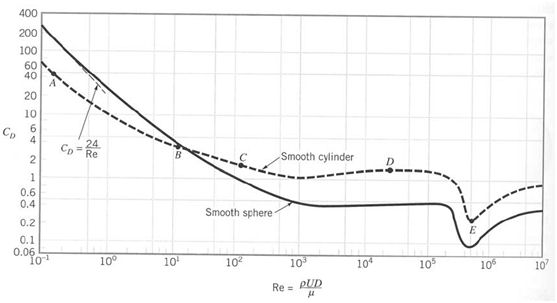
\includegraphics[width=1.0\textwidth]{figs/Shape_CoefficientC.jpg}
\caption{Drag coefficient as a function of Reynolds number for a smooth cylinder and a smooth sphere.  The linear approximation of $24/Re$ is also shown.}
\end{figure}
Therefore,
\begin{equation}
F_{\rm drag} = 12 \nu \rho_{\rm F} U A / l
\end{equation}
Substituting in the drag area of a sphere:
\begin{equation}
F_{\rm drag} = 12 \nu \rho_{\rm F} U \pi (d/2)^2 / l
\end{equation}
where $d$ is the particle diameter.
The force that balances the drag force is the buoyancy force:
\begin{equation}
12 \nu \rho_{\rm F} U \pi (d/2)^2 / l = \frac{4}{3} \pi \left(\frac{d}{2}\right)^3 g (\rho_{\rm S} - \rho_{\rm F})
\end{equation}
where $g$ is gravitational acceleration, and $\rho_{\rm S}$ is density of the spherical particle.  Rearranging:
\begin{equation}
U = \frac{gdl}{18 \nu} \left( \frac{\rho_{\rm S} - \rho_{\rm F}}{\rho_{\rm F}} \right)
\end{equation}
The fractional density difference due to thermal effects can be expressed as:
\begin{equation}
\frac{\rho_{\rm S} - \rho_{\rm F}}{\rho_{\rm F}} = \alpha \Delta T = \alpha l \left( \frac{dT}{dz} - \left( \frac{dT}{dz} \right)_{\rm s} \right)
\end{equation}
And finally, set the particle diameter equal to the length-scale parameter $l$, which is the mixing length:
\begin{equation}
U = \frac{\alpha g l^3}{18 \nu} \left( \frac{dT}{dz} - \left( \frac{dT}{dz} \right)_{\rm s} \right)
\end{equation}
%%%%
%%%%
%%%%
\subsubsection{Inviscid scaling}
For the inviscid case we follow \citep{V53}, with some additional insights from \cite[p. 50,][]{KWW12}.  Kinetic energy of a fluid element is balanced by the work done by the buoyancy force over some length scale $x$:
\begin{equation}
\frac{1}{2} m v^2 = \int_0^x K(x) dx
\end{equation}
where $x$ relates to the mixing length.  The buoyancy force is:
\begin{equation}
K(x) = V g \Delta \rho(x) = m g \alpha \Delta T(x)
\end{equation}
where $V$ is volume of the element, $g$ gravity, $\Delta \rho$ density anomaly, $m$ mass of the element, $\alpha$ thermal expansion coefficient, $\Delta T$ thermal anomaly:
\begin{equation}
\Delta T(x) = \left( \frac{dT}{dz} - \left( \frac{dT}{dz} \right)_s \right) x
\end{equation}
Now we can integrate:
\begin{equation}
\int_0^x K(x) dx = mg \alpha  \left( \frac{dT}{dz} - \left( \frac{dT}{dz} \right)_s \right) \frac{x^2}{2}
\end{equation}
Putting this together with the kinetic energy \citep[Eq.~5,][]{V53}:
\begin{equation}
v(x) = \sqrt{\alpha g x^2 \left( \frac{dT}{dz} - \left( \frac{dT}{dz} \right)_s \right)}
\label{eq:mixvele}
\end{equation}
This establishes the basic form of the inviscid scaling for velocity, minus the factors of two that are now discussed.  \cite{V53} then computes an average velocity of all the parcels of fluids with different mixing lengths that are passing through the same region:
\begin{equation}
\overline{v} = \frac{\int_0^l v dx}{\int_0^l dx} = \sqrt{\frac{\alpha g l^2}{4} \left( \frac{dT}{dz} - \left( \frac{dT}{dz} \right)_s \right)}
\end{equation}
This agrees with \cite[Eq.~6a,][]{V53}.  Note that in \cite{V58} she increases the factor from 4 to 8 to improve the description of the turbulent friction \citep[see][]{B98}.  \cite{HVB65} actually look at values up to 16, which may perhaps be the origin of the factor of 16 in \cite{ABE93,ABE95}?  Other origins for factors of two include considering the average thermal perturbation of an element over $[0,x]$:
\begin{equation}
\overline{\Delta T} = \frac{\int_0^l \Delta T dx}{\int_0^l dx} = \left( \frac{dT}{dz} - \left( \frac{dT}{dz} \right)_s \right) \left( \frac{l}{2} \right)
\end{equation}
\cite{KWW12} consider an ``average'' element from the start of their derivation, and thus introduce a factor of two through the average path length of $l_m/2$, which first appears in the thermal anomaly.  Second, another factor of two appears since the buoyancy force is integrated over the average path length.  Finally, another factor of two appears since they assume that half of the work goes into the kinetic energy of the element.  Hence \cite{KWW12} end up with a factor of 8 in the denominator, albeit by slightly different reasoning.  Although \cite{ABE93,ABE95} reference \cite{V53}, it's not obvious that you can just use \cite{V53} and arrive with a factor of 16 in the denominator.  Since factors of 2 seem to be introduced for a variety of reasons by different authors, with origins that are not necessarily explained well, we may just have to accept that \cite{ABE93,ABE95} uses a factor of 16 in the denominator by appealing to a combination of the reasons previously described.  In the end, the numerical challenges result from the presence of the square-root and not the constant prefactor:
\begin{equation}
v_{\rm invis} = \sqrt{\frac{\alpha g l^2}{16} \left( \frac{dT}{dz} - \left( \frac{dT}{dz} \right)_s \right)}
\end{equation}

%%% added Rob Spaargaren as part of his MSc work
\subsection{Kamata and Wagner profile}
According to Kamata (2018) and Wagner et al.\ (2019), the classical mixing length profile is not able to reproduce realistic results, with Nusselt number and average temperature deviating by up to 60\% from 3D simulations. They came up with a way of parametrizing the mixing length profile to get more realistic results. For mantle thickness $D$, the profile can be characterized by two parameters: depth $a$ and size$b$, where the peak of the profile is at a depth of $a\cdot D$ km, and the size of the peak is $b \cdot D$ km. The profile consists of two linear lines from 0 at the top and bottom of the mantle to the peak of the profile. In the classical MLT, we have $a=b=0.5$. Kamata (2018) and Wagner et al. (2019) varied these numbers in their simulations to see which sets gives the most representative results.

\subsubsection{Kamata's results}
Kamata (2018) finds that the coefficients $a$ and $b$ depend on two parameters: relative mantle size $f = R_{CMB}/R_{top}$, which is about 0.55 for Earth (and is an input parameter for SPIDER), and viscosity contrast across the mantle $\gamma = \ln (\eta_{top}/\eta_{bottom})$.  His descriptions for the parameters are quadratic equations of $f$, $a,b = a_2,b_2 f^2 + a_1,b_1f + a_0,b_0$, where the coefficients depend on $\gamma$. (see equations 13-20 in his paper). He finds that the coefficients slightly depend on the Rayleigh number of the system, but not significantly enough to include it in the parametrization (see Figure 4 in his paper).

\subsubsection{Wagner et al.'s results}
Wagner et al.\ (2019) use a different parametrization in terms of $\alpha$ and $\beta$, which can be transformed to the original coefficients as $a = \beta/2$ and $b=\alpha/2$. They find a more complex relationship, which depends on the viscosity contrast and on the Rayleigh number of the system. They present a scaling law in their Figure 7 and Table 4,
\begin{equation}
\alpha = \left( a_0 - a_1 \gamma - a_2 \log(\text{Ra}) \right) \tanh \left( a_3 \log (\text{Ra}/\text{Ra}_c) \right),
\end{equation}
where Ra$_c$ is the critical Rayleigh number (which they present an approximation for as a function of $\gamma$). Their parametrization of $\beta$ depends on the dynamic regime. For the stagnant lid regime it is slightly simpler:
\begin{equation}
\beta = b_0 - b_1 \gamma - b_2 \log (\text{Ra}),
\end{equation}
while for the mobile and sluggish lids it's a more complex equation
\begin{equation}
\beta = b_0 - b_1  \tanh \left( \log(\text{Ra}) - b_2 - b_3 \gamma^{b_4} \right).
\end{equation}
Values for the numbers are given in their Table 4, for both Bottom-heated and Mixed heated models (as long as internal heating by radiogenic elements is switched on, we're in the mixed heating regime).
